\documentclass[conference,compsoc]{IEEEtran}
% \documentclass{IEEEconf} 
\usepackage{url}
% \usepackage{hyperref}
\usepackage{amssymb,amsmath}
\usepackage{pdfpages}
\usepackage{graphicx}


% \title{No solution? Clustering to Evaluate Multiple Imputation } 
% \title{CLEMI (CLustering to Evaluate Multiple Imputation: The Framework}
\title{CLEMI: A Proof-of-Concept Computational Framework for Clustering to Evaluate Multiple Imputation}
% \author{Anthony S. Chapman, Steven Turner, Wei Pang, Lorna Aucott} 
\author{
    \IEEEauthorblockN{Anthony Chapman\IEEEauthorrefmark{1}\IEEEauthorrefmark{2},
    				  Steve Turner\IEEEauthorrefmark{3},
    				  Wei Pang\IEEEauthorrefmark{1}, 
    				  Lorna Aucott\IEEEauthorrefmark{2}}
    \\ \IEEEauthorblockA{\IEEEauthorrefmark{1}School of Natural and Computing Sciences, University of Aberdeen, UK, AB24 3UE}
    \\ \IEEEauthorblockA{\IEEEauthorrefmark{2}Institute of Applied Health Science, University of Aberdeen, UK, AB25 2ZD}
    \\ \IEEEauthorblockA{\IEEEauthorrefmark{3}Child Health, University of Aberdeen, UK, AB25 2ZG}
}

\begin{document} 
	\maketitle{} 

	% \abstract{
	\begin{abstract}
	Introduction: Missing values are a problem for all researchers working with routinely acquired data. Using a benchmark created from a subset of the original values consisting of the complete cases and computing clustering techniques \cite{clustering} we are able to create a program to evaluate the effect of imputing missing values. This paper describes an imputation evaluation algorithm, called ClEMI (Clustering to Evaluate Multiple Imputation), which returns a score for that researchers can use. 

	Methods: A benchmark is created from the complete cases of a dataset and then testing datasets are created from the benchmark. Imputing all datasets and using clustering to find the dissimilarity between the dataset we are able to find the effect of imputing missing values.
	
	Results: We tested ClEMI in two different ways to find how different amounts of missing values affect imputation. We found that a dataset should have between 40\% to 70\% of the records with missing values. We also found that for a dataset with missing values each individual records should not have more than 40\% of the values missing for imputation. 
	
	Conclusion:
	The testing carried out in this paper is dataset specific, we found that for our dataset, we should only include records with 60\% or more of the values present for imputation before any analysis. These results may be different for other datasets and ClEMI should be used to find such results.

	\end{abstract}	
	% } An abstract is usually ~250 words and includes introduction, methods, results and conclusion.

	\section{Introduction} % (fold)
	\label{sec:introduction}
	% Introduction – what is known (ie your recent presentation to Pang and Lorna, missingness is a problem)  what needs to be known (when is it appropriate to use MICE?) and what you are going to do about it (provide objective measures of “goodness-of-fit”)

	Missing data are a renowned challenge affecting big data analysis across the world. Data are missing due to many reasons, ranging from human error, unforeseen circumstances (most commonly due to participants of studies dropping out), hardware malfunctions and even software problems \cite{pigott2001review}. Some current systematic reviews of cohort studies \cite{systematic1,systematic2,systematic3} show how different researchers dealt with missing data. The majority (circa 70\%) of the studies used complete case analysis (meaning records with missing values were not used for the analysis), and some (circa 25\%) do not mention whether there were any missing values or what they did if there were. 

	Although there are ways to combat missing data, such as mean-value imputation or multiple imputation \cite{missing1,missing2,missing3}, it is still considered acceptable to perform complete case analyses \cite{systematic1,systematic2,systematic3}. Imputation techniques, such as MICE (Multivariate Imputation by Chained Equations) \cite{MICE}, could improve any results by using more of the available data. As an example, in \cite{epi1}, the authors use only 2,758 records for analysis out of the possible 44,261 mainly due to missing data. MICE is a imputation program, written in the computing language R \cite{r}, one of the main advantages from MICE is that it uses all of the available data to form probabilistic models of what the missing values could be, it then creates several datasets which differ slightly and pools them together for a single imputed dataset.

	Some of of the main reasons why complete case analysis is carried out for research are: researchers are uncomfortable with imputation software and/or it is difficult to evaluate an imputation method on a specific datasets. This paper focuses on a possible solution to these two problems, an imputation evaluation program that works on a wide range of datasets.

	Clustering \cite{clustering,clust-char}is a computational method of grouping records in a dataset with other similar records, the idea being that all records in one grouping (a cluster) will be more similar to any point in the same cluster than any other point in other clusters. We will use clustering to calculate the dissimilarity between datasets, doing so we will be able to treat a dataset as a multidimensional point in a higher dimensional plane, thus if we have several datasets, they will be several points in the plane and one can calculate the dissimilarity. Clustering a clusterings have characteristics which can be used to calculate the dissimilarity between datasets, such characteristics include (but do not exhaust): cluster sizes (amount of points in a cluster), cluster widths (how different points in a cluster are from other points in the same cluster) and cluster isolation (how densely packed each cluster is). Using these characteristics, we will be able to quantify the difference between distinct datasets. 

	Our objectives are as follows: 1. To create a program that shows the impact of applying an imputation method to a dataset with missing data. 2. To evaluate the limitations of the program by using artificially incomplete datasets which are created from a complete dataset, we will be able to compare the effect by comparing datasets. 3. To test the program on a real dataset. The first objective will be achieved by using a benchmark (obtained from the dataset to be imputed) dataset and clustering techniques to find the dissimilarity between an imputed dataset and it's true values. The program should be able to cope with a variety of extremely high dimensional and sparse dataset and it should be able to reliably output an efficiency score with nothing more than the users initial imputes of a dataset and imputation method. 

	For the second objective, we will use our program in two different ways. Firstly, we will systematically remove amounts of variables from a testing dataset to create new datasets, each one with a larger amount of records with missing values. Applying the software to these new datasets, we will be able to see the effect different amounts of missing records have on MICE.

	Finally, a real dataset with missing values will be used to see how different levels of missing values with each records affect imputation, for example, should we impute records with 7 missing values and 3 recorded values. We will create more datasets where we ignore any records with a certain amount of missing values, for example dataset 1 will have all records with 90\% or more values present, dataset 2 will have all records with 80\% or more values present, all the way to 10\% values or more. Applying our software to all these datasets, we will be able to judge which records we allow in the dataset for analysis.




	% section introduction (end)

	\section{Methods} % (fold)
	\label{sec:methods}
	% Methods – what you did.  This is a bit dull and should read like a recipe and allow the reader to replicate what you have done
	This section will: Describe ClEMI, our imputation evaluation software in Section~\ref{sub:clemi}. Evaluate ClEMI by creating incomplete datasets from a testing dataset in Section~\ref{sub:evaluating_clemi_on_volume_of_missing_data}. Use ClEMI on a real dataset to find the optimal amount of missingness one should allow before imputing the dataset in Section~\ref{sub:evaluating_clemi_on_volume_of_missing_data}.

	\subsection{ClEMI} % (fold)
	\label{sub:clemi}
	
	The underlying concept of the program is to create a benchmark dataset from the complete records, then create artificially missing datasets which represent the original dataset out of the benchmark by mimicking the missingness of the original dataset. We achieve this by analysing the pattern of data missing for a specific dataset and create testing datasets by imposing the same missingness into the benchmark. We then impute the artificially missing datasets, using MICE, and analyse how far they have deviated from the benchmark. We can then check how far MICE takes the artificial datasets from the benchmark by using clustering techniques. We now provide a step by step guide on how our program will work, we will call the dataset to be imputed $O$.
	\\
	\indent \textbf{Stage 1: Extracting a Benchmark}
	Firstly, a benchmark needs to be created, this can be done by extracting the complete records from the dataset; call this benchmark dataset $CC$ for Complete Cases. $O$ can then be analysed to find the missingness characteristics, these will be used to create testing datasets later in the process. Notice that $CC$ is a subset of $O$ 
	\begin{figure}[!ht]	
		\caption{Stage 1: Create a benchmark dataset by extracting the complete cases from the original dataset.}
		\centering
		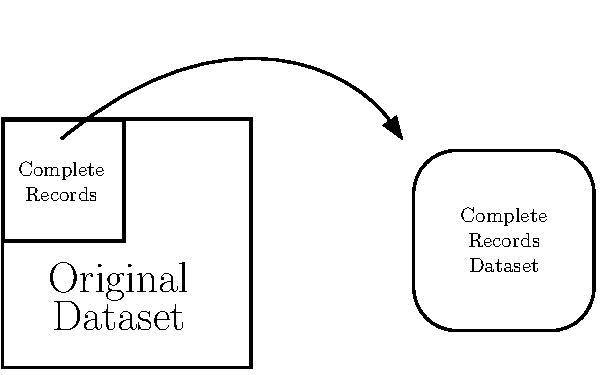
\includegraphics[width=0.35\textwidth]{stage1.pdf}
	\end{figure}
	\\
	\indent \textbf{Stage 2: Create Dummy Datasets}
	Next, artificially incomplete datasets are created, called $artMiss.i$ where $i$ is a number from 1 to $n$, by applying the missingness characteristics from $O$ to $CC$ $n$ times. We do this by finding the amounts of missing values and proportionally deleting values from $CC$ in accordance to the missing characteristics of $O$. It is important to apply the missingness in a manner that treats each $artMiss.i$ separately; doing so will aid in a more robust test. Thus we now have a benchmark dataset $CC$, and $n$ artificial datasets with missing data which follow the same missingness structure as the original dataset.
	\begin{figure}[!ht]
		\caption{Stage 2: Create artificially incomplete datasets by mimicking the amount of missingness of the original onto the benchmark.}
		\centering
		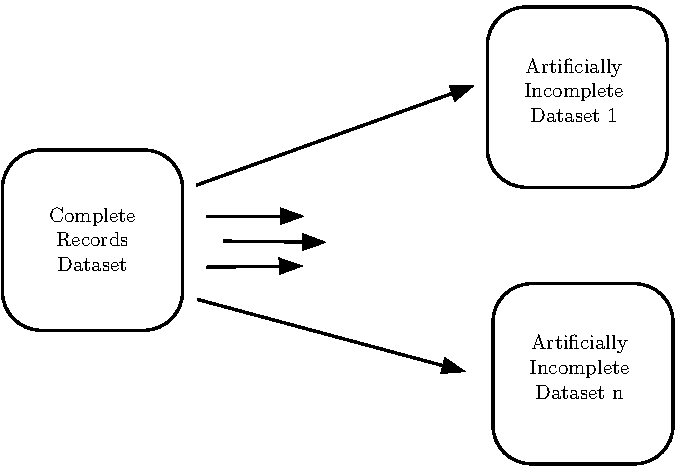
\includegraphics[width=0.35\textwidth]{stage22.pdf}
	\end{figure}
	\\
	\indent \textbf{Stage 3: Impute Dummy Datasets}
	The next step will be to impute all $artMiss.i$ with our chosen imputation method, it is important to apply exactly the same procedure (same imputation with the same parameters) to all datasets in order to have reliable results. This will create $n$ artificially complete (imputed) datasets, called $artComp.i$ where $i$ ranges from 1 to $n$. 
	\begin{figure}[!ht]
		\caption{Stage 3: Impute all artificially incomplete datasets.}
		\centering
		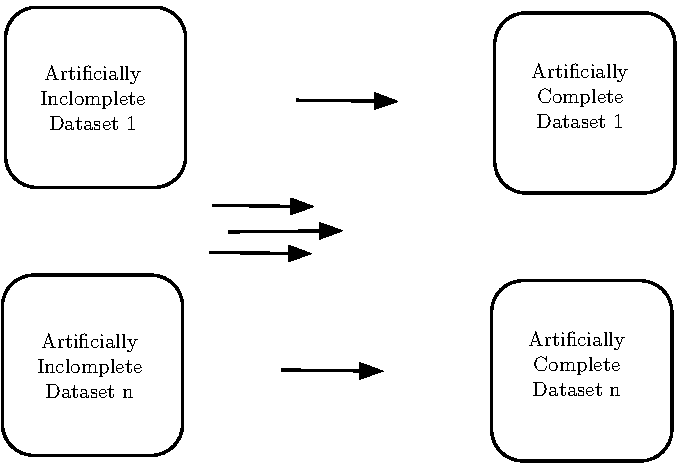
\includegraphics[width=0.35\textwidth]{stage3-2.pdf}
	\end{figure}
	\\
	\indent \textbf{Stage 4: Cluster all Datasets}
	By using clustering techniques one can evaluate the difference between all $artComp.i$ and $CC$. By finding the difference between sets of clusters; one can see how close (or far) an imputation method has taken each $artMiss.i$ from the true values (the benchmark $CC$). It will now be possible to compare the effect of different imputation methods.

	Thus it is needed to cluster our benchmark dataset $CC$ and all imputed datasets $artComp.i$, $clustCC$ will be the clustering of $CC$ and $clust.i$ will be all clustered $artComp.i$. Note that as with imputing all datasets one needs to make sure the same clustering method with the same parameters are being used on all datasets. This way one can reliably calculate the difference between clusterings.
	\begin{figure}[!ht]
		\caption{Stage 4: Apply a clustering algorithm to all the imputed datasets.}
		\centering
		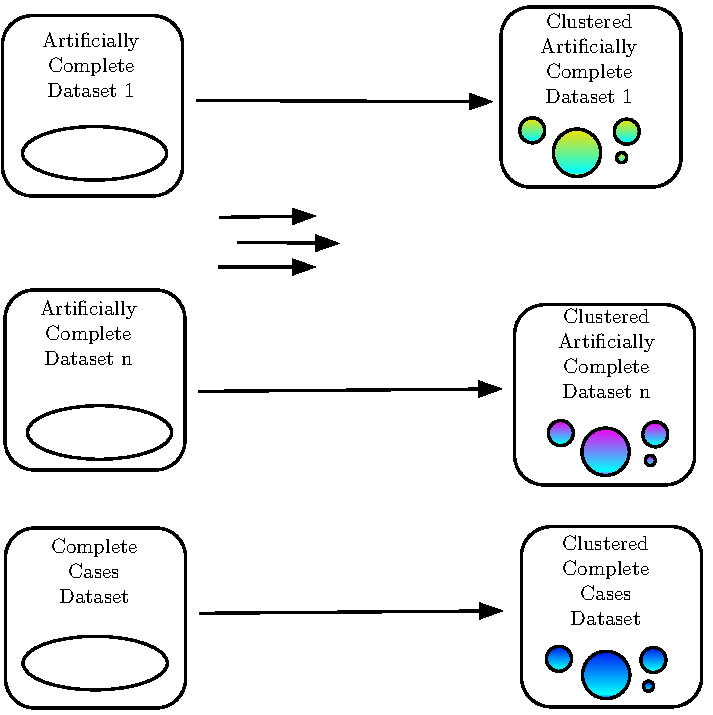
\includegraphics[width=0.35\textwidth]{stage4-2.pdf}
	\end{figure}
	\\
	\indent \textbf{Stage 5: Distance Function Between Artificial Datasets and Benchmark}
	Finally, calculate the distance between all $clust.i$ and $clustCC$. This will indicate the effect of imputing an incomplete dataset by finding the distance between the clustering of the imputed datasets ($clust.i)$ and the clustering of our benchmark ($clustCC$). The system should output an efficiency indicator, at the end of the process, to show how far away all $clust.i$ are from $clustCC$; this will be how the user judges whether an imputation method gives correct values or not. Whether the final output describes a successful or efficient imputation method will be subjective. The output should be a normalised result in order to make comparison with other imputation outcomes clearer. The aim is to make it easier for all researchers to see the effect of imputation and feel more confident in using data with imputed values for analysis.

	It will be up to the researcher to decide whether the imputed values are close enough to represent the truth or whether they are too far to provide fair results from any type of analysis.
	\begin{figure}[!ht]
		\centering
		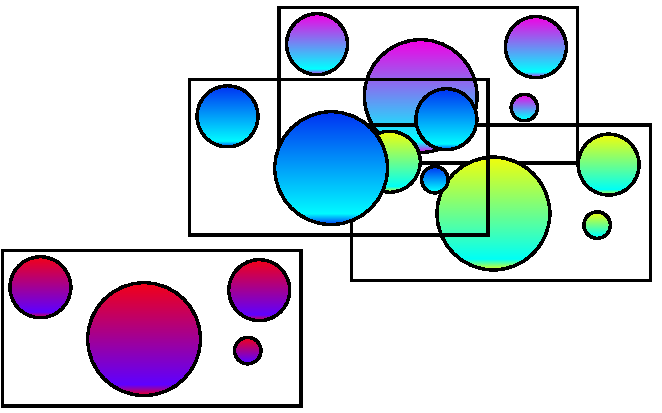
\includegraphics[width=0.35\textwidth]{stage5-2.pdf}
		\caption{Stage 5: Using the clustering characteristics find the dissimilarity between all imputed datasets and the benchmark.}
		\label{fig:stage-5}
	\end{figure}

	Figure \ref{fig:stage-5} is a visual representation of what comparing different clustered datasets looks like. Each box represents a clustering and contain a set of clusters. Using clustering characteristics, one can compare clusterings and evaluate whether clustering A is more similar to clustering B than it is to clustering C is.
	\\
	\indent \textbf{Stage 6: The Output}
	In our implementation, described above, produces six scores, three for MICE and three for mean imputation, as a reference point. Each set of three consists of one cluster sizes score, one cluster widths (how wide each cluster is) score and one isolation (how dense the clusters are) score, ClEMI can then output a set of three graphs to visualise these scores. The first graph will be the cluster size scores, the second graphs will show the individual cluster width scores and the third graph the isolation scores. A blue line will represent the imputation scores and the red line is mean imputation. In each graph the y-axis represents the score and the x-axis shows the amount of missingness. 

	% subsection clemi (end)
	\subsection{Evaluating ClEMI on Volume of Missing Data} % (fold)
	\label{sub:evaluating_clemi_on_volume_of_missing_data}
	In order to find the limitations of imputing large amounts of missing data, we obtained a dataset and created testing datasets by removing varying amounts of records, this induced missingness will be used to test MICE's performance in different situations. We obtained a testing dataset from a machine learning repository \cite{forestFires}, a well recognised data bank for testing machine learning techniques. Our chosen dataset, called ForestFires, consists of 517 rows with 13 variables and is freely available,  it was chosen as it is big enough to produce reliable results but small enough so that we can run it many times. 9 testing datasets were created from the testing dataset by selecting a specified percentage of records and removing a random amount of values from each record, the testing datasets start at 10\% missing records and go to 90\% missing records with 10\% increments. We then applied CLEMI to each dataset and plotted the results on a single graph to compare the results. The test will be run 10 times and the outcomes where averaged from all tests can be seen in the graphs in Figure~\ref{fig:clemi-limit}.  

	% subsection evaluating_clemi_on_volume_of_missing_data (end)

	\subsection{Using ClEMI to Find a Missingness Threshold} % (fold)
	\label{sub:using_clemi_to_find_a_missingness_threshold}
	When imputing a dataset, we need to know how much missingness should be included. For example, there might be no benefit from imputing an empty record. To know how much missingness we include for imputation we need to find a missingness threshold. We use a sample dataset from the Seaton Cohort \cite{seaton}, we will call this ABDN, with 2000 records, 8 variables per record and a large amount of missing data shown in Figure~\ref{fig:missing}. We created 9 new datasets, the first dataset contains all records with 10\% or less missing values in each record (mostly complete records), the second with 20\% or less missing values and so on until 90\% or less missing values per record (almost all records from the original dataset). We then applied ClEMI to each dataset and plotted the results on a single graph to compare the results. The test was run 10 times (for time constraints) and the averages from all tests can be seen in the graphs in Figure~\ref{fig:clemi-limit2}.
	\\
	\begin{figure}[!ht]
		\centering
		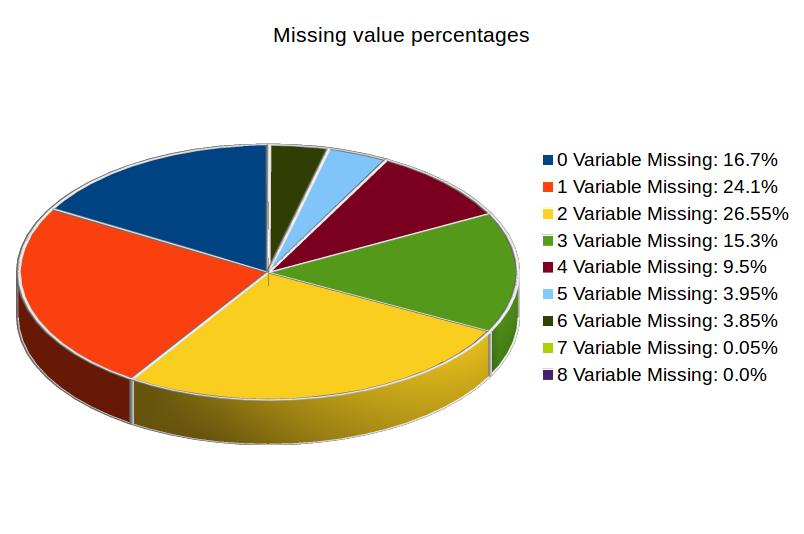
\includegraphics[width=0.40\textwidth]{missing-perc-equal}
		\caption{Amount of missing data - key on the left shows the \% of records with a specific amount of missing values. 0 variables missing: 16.7\% means there is roughly 17\% complete records.}
		\label{fig:missing}
	\end{figure}
	% subsection using_clemi_to_find_a_missingness_threshold (end)

	% section methods (end)

	\section{Results} % (fold)
	\label{sec:results}
	% Results – What your findings were.  This is essentially point 2 above.  You are scientifically testing your software and validating the findings
	The results are split into the two tests carried out, firstly, we evaluated how different amounts of missing data affect ClEMI and secondly, we use ClEMI to find how much missingness one should allow when imputing a dataset which will be used for further analysis.

	\subsection{Evaluating ClEMI} % (fold)
	\label{sub:evaluating_clemi}
	The scores seen in Figure~\ref{fig:clemi-limit} show that MICE performs well when 40\% to 75\% of the records have missing values. This test does not take into account how many values per record are missing, it looks at the volume of records with missing values. From the graphs we can see that if a dataset has less than 40\% missingness MICE will perform well but not as well as if it had 40-75\% missingness. Similarly we can see that if more than 75\% of the records are missingness, then MICE performs even worst.
	\\
	\begin{figure*}[!ht]
		\centering
		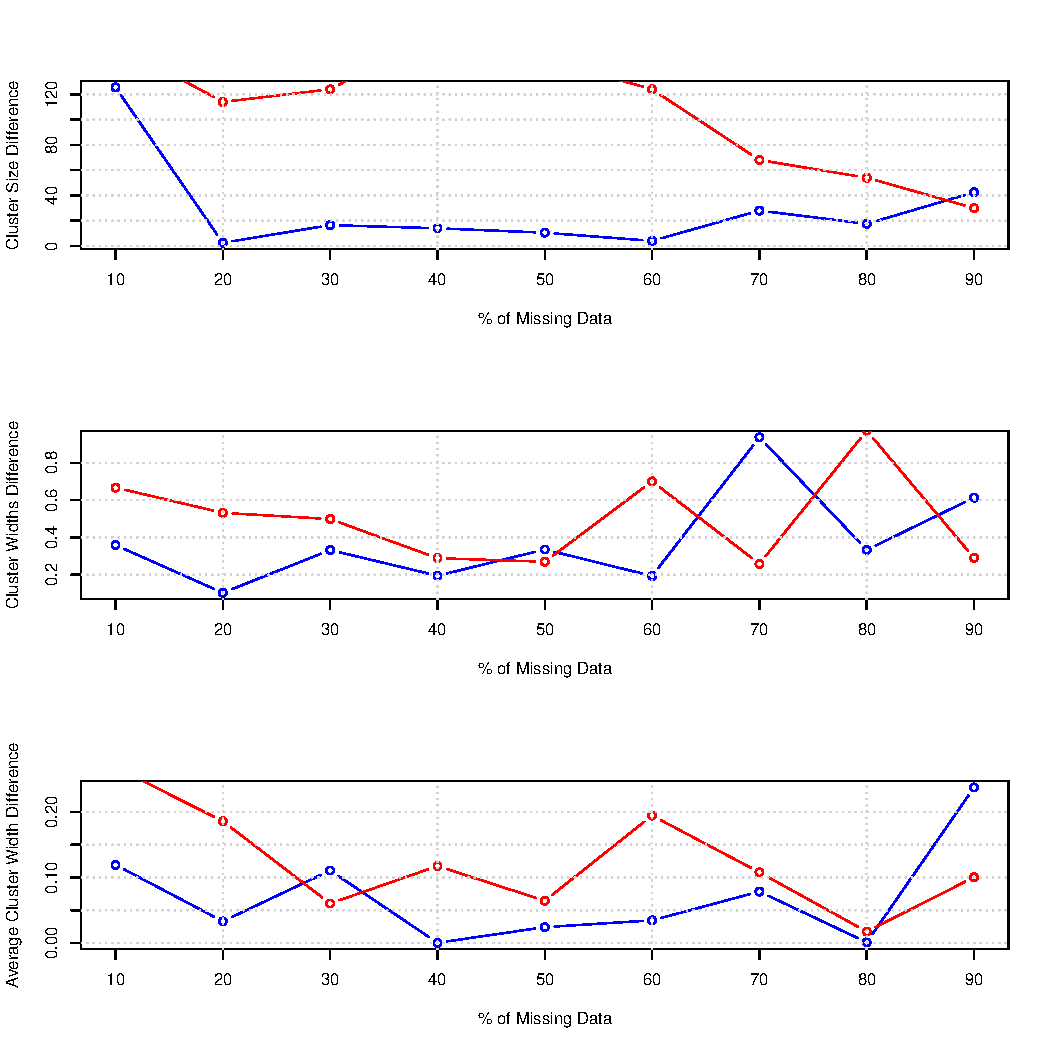
\includegraphics[width=\textwidth]{forestFires}
		\caption{CLEMI test 1 - Cluster size score, Cluster widths score and Cluster isolation score. }
		\label{fig:clemi-limit}
	\end{figure*}	
	% subsection evaluating_clemi (end)

	\subsection{Missingness Threshold} % (fold)
	\label{sub:missingness_threshold}
	The scores seen in Figure~\ref{fig:clemi-limit2} show that we should not include records with less than 65\% of their values missing for imputation. From our ADBN dataset, we should only impute records with 5 or more known values (out of a possible 8). As you can see in Figure~\ref{fig:missing}, we will be able to use circa 75\% of the available records for imputation and then analysis, compared to circa 17\% if we carried out a complete case analysis. 
	\\
	\begin{figure*}[!ht]
		\centering
		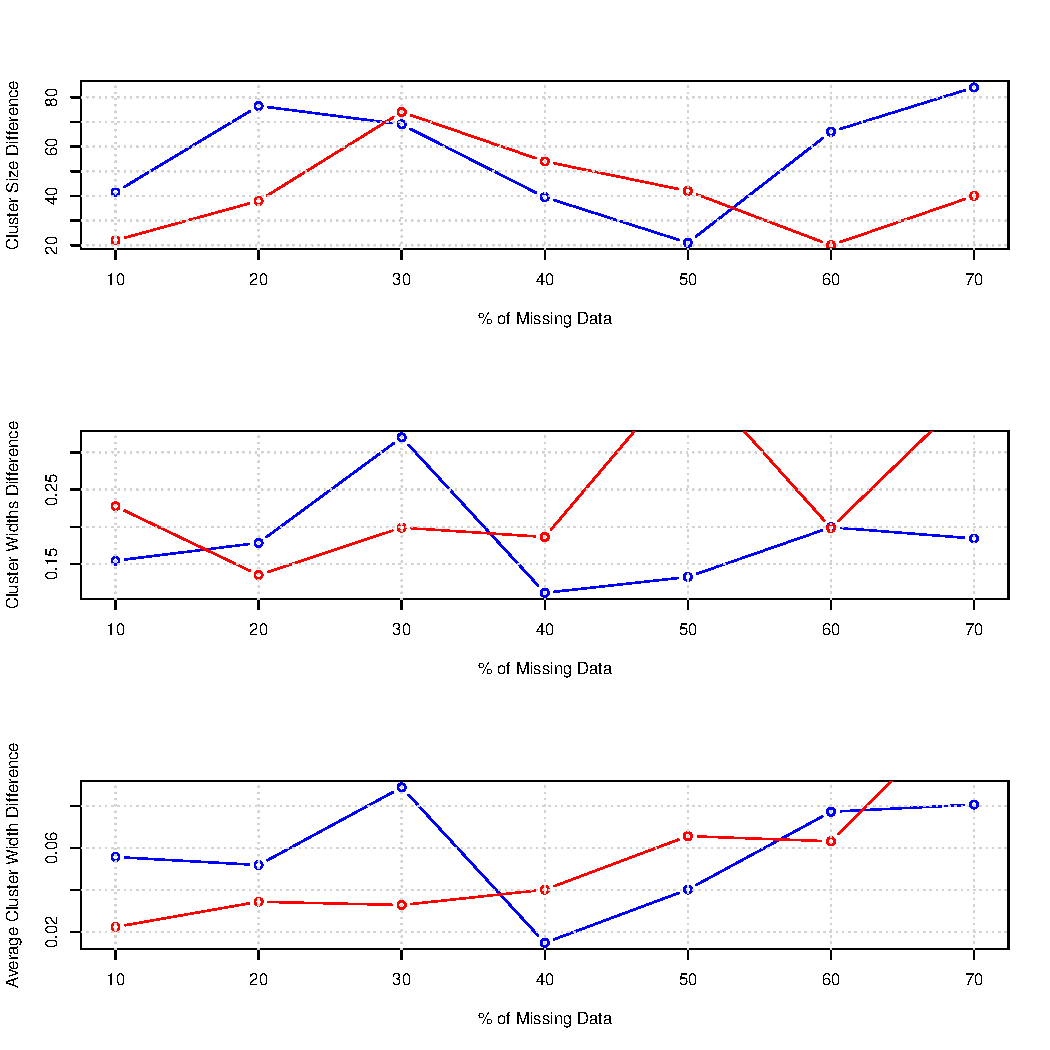
\includegraphics[width=\textwidth]{AMND4}
		\caption{CLEMI test 2 - Cluster size score, Cluster widths score and Cluster isolation score. }
		\label{fig:clemi-limit2}
	\end{figure*}
	
	% subsection missingness_threshold (end)



	% Figure~\ref{fig:clemi-limit2} shows 


	% section results (end)

	\section{Discussion} % (fold)
	\label{sec:discussion}
	% Discussion – four parts (i) summary of the main findings (ii) comparison with what is already known, what does your work add to the literature? (iii) how the software works and what is is actually doing (iv) strengths and limitations.
	Firstly, we found MICE performs better when the ForestFires dataset contains 40\%-70\% records with missing values. We also note that, less that 40\% missingness can be imputed with a better score than a dataset with greater than 70\% missingness. By noticing that MICE works by making probabilistic models from both the data that is complete and the data that is partially missing we realised that if there is small amounts of missing data, then the probabilistic model does not have enough data to accurately predict the values that are missing. 

	Our second finding, to find a missingness threshold, only applies to our ABDN dataset, this method can be used to any dataset and the results are dataset specific. We found that imputing records with more than 65\% missing values it may affect any analysis negatively by creating wrong values. The test shows that only records with 65\% or more known values should be allowed to be imputed and then used for analysis.

	% Although there has been previous work on evaluating an imputation method on a specific dataset \cite{eval1,eval2}, they have not created a program to do it autonomously. We have created a program researchers could use, regardless of their field of interest. This software could also be used to find interesting general traits of imputing data, such traits would include imputing many datasets with missing values and storing the results. These results can be used to give rough estimates on imputation without using ClEMI. 

	The main strengths of ClEMI are that it can be used to optimise MICE, by changing how much missingness is allowed in the study and changing the imputation parameters, one is able to have more reliable dataset for analysis, thus more reliable results. 

	ClEMI's main limitation is that the interpretation of the results are subjective, ClEMI outlines the distance between an imputed dataset and its original form. It does not guarantee that a dataset can be imputed and is only an estimation on whether an imputation method will successfully impute a dataset or not. Other limitations are that we only carried each test 10 times and averaged the results, in the future it will be beneficial to carry out the same tests over 100 or even 1,000 times and use the averages from that. We also need to create testing dataset with other types of missingness rather than at random. 
	
	By addressing the objectives stated in Section~\ref{sec:introduction} we hope to make imputation more accessible to researchers who currently analyse only complete datasets, as well as make the results from imputed data analysis more credible by evaluating the imputation method prior to any analysis. % Finally, the program could also be used to assess whether a given dataset can be imputed or not. 	

	\section{Future Work} % (fold)
	\label{sec:future_work}
	Being able to use ClEMI with more imputation methods than just MICE would provide us with a way to reliably compare different imputation methods using ClEMI's output score. This could make sure that a dataset can be imputed with the most appropriate method and thus give a more reliable outcome after analysis. 

	It would be good to use the same methods as already described on other datasets. By analysis large amounts of datasets, we will be able to find more generally, how different types of missing data affect imputation.  By using other datasets with different types of missing data we will be able to build a bigger picture. 
	% section future_work (end)

	\bibliographystyle{IEEEtran}
	\bibliography{papers}

\end{document}




A receiver operated characteristic curve will be used to determine the CRL z score with best sensitivity and specificity for outcomes. For asthma severity (measured on ordinal scale of 1-5 and based on treatments prescribed) we will use ordinal logistic regression.



You can look at any cohort study you chose Anthony!  What might be more meaningful is to look at a number of systematic reviews on a topic and then look at the completeness of data within each review.  This will give you 4-5 references which encompass up to 100 original papers.  I attach a SR on asthma aetiology.  You could look for SRs on other non-communicable diseases in  childhood (and ideally the ones you are going to look at, eg obesity, epilepsy, ADHD and diabetes).
 
Best wishes
Steve